\documentclass{jarticle}
\usepackage{mathtools, multicol}
\usepackage{color}
\usepackage{url}
\usepackage{comment}
\usepackage{here}
\usepackage{txfonts}
\usepackage{listings, jlisting}
\usepackage{latexsym}

\renewcommand{\lstlistingname}{リスト}

\lstdefinestyle{customplain}{
  belowcaptionskip=1\baselineskip,
  breaklines=true,
  frame=tRBl,
  xleftmargin=\parindent,
  language=,
  showstringspaces=false,
  numbers=left,
  basicstyle=\footnotesize\ttfamily,
  keywordstyle=\bfseries\color{black},
  commentstyle=\itshape\color{black},
  identifierstyle=\color{black},
  stringstyle=\color{black},
}

% 余白の設定
\usepackage[top=20truemm, bottom=16truemm, left=10truemm, right=10truemm]{geometry}

% 図の挿入
\usepackage[dvipdfm]{graphicx}

% より複雑な数学記号
\usepackage{amsmath,amssymb}

% 図の通し番号
\usepackage{subfigure}

\newcommand{\todayd}{%
\the\year.{\ifnum \month < 10 0\the\month \else \the\month \fi}.%
{\ifnum \day < 10 0\the\day \else \the\day \fi}}


\makeatletter

\def\@thesis{人工知能}
\def\id#1{\def\@id{#1}}
\def\department#1{\def\@department{#1}}

\def\@maketitle{
	\begin{center}
		{\huge \@thesis \par} %大きなタイトルが記載される部分
		\vspace{10mm}
		{\LARGE\bf \@title \par} % タイトル部分
		\vspace{20mm}
		{\Large 提出締切: 2013.11.21\par} % 提出年月日部分
		\vspace{5mm}
		{\Large 提出日:  \@date \par} % 提出年月日部分
		\vspace{20mm}
		{\Large \@department \par} % 所属部分
		\vspace{10mm}

		{\Large\@id } % 学籍番号部分
		{\Large \@author} % 氏名 
	\end{center}
\par\vskip 1.5em
}

\makeatother

\title{第3回講義課題 課題番号07}
\date{\todayd}
\department{工学部電子情報工学科}
\id{03-123006}
\author{岩成達哉}


\begin{document}

\begin{titlepage}
	\setlength{\topmargin}{1.1in}
	\vspace{100mm}
	\maketitle
\end{titlepage}


\section{EvansのプログラムANALOGYによる幾何図形類推問題}
本課題では,図\ref{fig:charts}の例を用いて解説を行う.問題は忠実に,「Aを変えてBにする規則をみつけ,それをCに適用せよ. その結果できる図形を1〜5から選べ」を採用する.この問題の答えの導出は,周囲の4つの図形のうち,3つある同じ図形の1つだけを拡大し,中心の図形を縮小してその中に収める.周囲の他の図形は削除する.図形の色は塗りつぶしがあれば塗りつぶしをやめ,塗りつぶされていなければ塗りつぶす.よって,この規則をCに適用して4の日の丸図形が答えである.

\begin{figure}[H]
	\begin{center}
	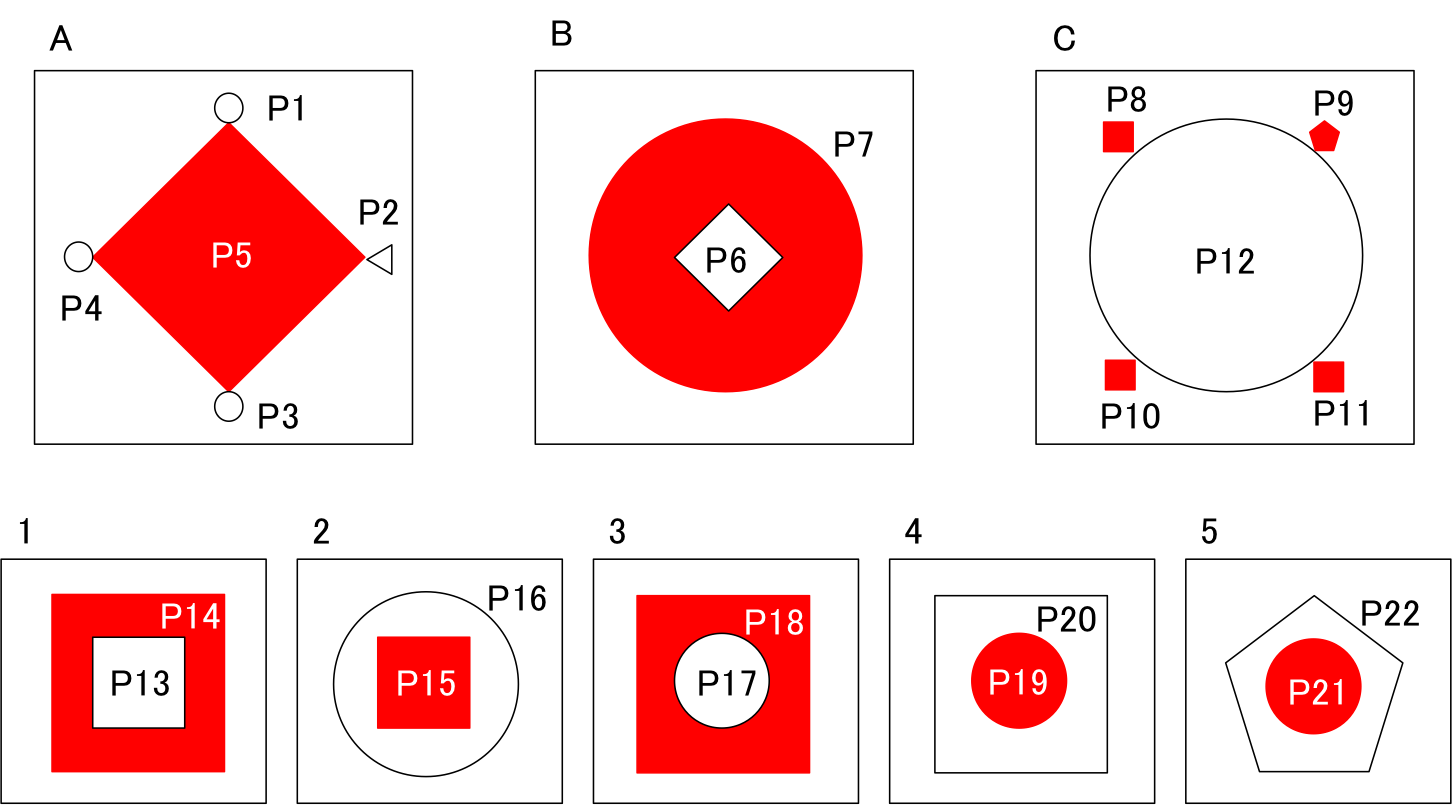
\includegraphics[width=13cm]{image/charts.png}
	\caption{題材とする幾何図形類推問題}
	\label{fig:charts}
	\end{center}
\end{figure}





\subsection{ANALOGYによる解法}
%EvansのプログラムANALOGYがどのようにこのような問題を解くことができたかを 説明せよ。次のような点を例をもとにして解説すること。 上以外の例を用いても良い。より面白い例の方が ポイントが高い。

ANALOGYによる上述の問題の解法を示す.EvansのANALOGYは,図形の記述と変換の記述を主に手動で行うプログラムであった\cite{ref:automation}.したがって,記述の例は複数存在する.これによって,意図的に正解にたどり着きやすい記述をしておくことが可能となる.\textcolor{red}{本課題では,図の記述と図の類似点の導出までを手動で行うと仮定し,変換規則の導出以降は機械的な手続きで行われるものとする.}

図の記述は以下のように定めた.
\begin{itemize}
\item FIG-*は図*の意
\item CONSISTS-OFは構成オブジェクトの一覧を示す
\item OBJECTSはそれぞれのオブジェクトの形を定義する
	\begin{itemize}
	\item ASSIGN a b\\
		オブジェクトaはbのような図形
		\begin{itemize}
		\item CIRCLE\\
			円
		\item TRIANGLE\\
			三角形
		\item SQUARE\\
			正方形
		\item PENTAGON\\
			五角形
		\item COMPOUND\\
			複雑な図形
		\item FILL a\\
			図形aを塗りつぶした図形
		\item ROTATION a b\\
			図形aを反時計回りにbだけ回転した図形
	\end{itemize}

	\end{itemize}
	\item RELATIONSはオブジェクト同士の関係を示す
	\begin{itemize}
	\item ABOVE a b\\
		aがbの上にある
	\item LEFT a b\\
		aがbの左にある
	\item INSIDE a b\\
		aがbの中にある
	\end{itemize}
\end{itemize}

これに従って,A,B,Cの記述を行う.これは,例えばリスト\ref{code:description}のようになる.
\lstset{style=customplain}
\lstinputlisting[caption={A,B,Cの記述},label=code:description]{source/description_abc.txt}





%A,B,C間の類似点と相違点とを記述するプログラムでは、これらの 各図をどのように記述しておけばよいだろうか?
さらに,A,B,Cに含まれる図形の類似関係を記述する.類似関係の記述は以下のように定めた.
\begin{itemize}
\item SIM-a-b\\
	図aと図bとの類似関係を示す
\item SIM a b:\\
	図形aと図形bとの類似関係を":"以下で示す
	\begin{itemize}
	\item TRANS c d e f\\
		図形aを
		\begin{itemize}
		\item cだけ拡大
		\item 反時計回りにdだけ回転
		\item eは対称性(N=なし,V=垂直軸対称,H=水平軸対称,P=点対称)を表す
		\item fは塗りつぶし切り替え(F=切り替えなし,T=切り替えあり)
		\end{itemize}
	\end{itemize}
\end{itemize}

すると,AとB,AとCの類似関係はリスト\ref{code:similarity}のようになる.AとBでは,P1〜P4はすべてP7と類似であり,P5はP6と類似である.ここで,「それぞれの図の間で一対一の類似関係を成り立たせること」を前提とし,P1とP7の類似関係のみ記述した.一方,AとCでは,図形の形としては同様のものはないとした.
\lstset{style=customplain}
\lstinputlisting[caption={AとB,AとCの類似関係の記述},label=code:similarity]{source/similarity.txt}





%図Aを図Bに変える規則の記号的な記述を与え、この規則を上で与えた記述からどのように機械的につくることができるかを説明せよ。
続いて,AをBに変形する規則を記述する.変形の記述方法を以下のように定めた.
\begin{itemize}
\item ADD a SHAPE b TO c\\
	オブジェクトaを図形bの形で条件cを満たすように追加する
\item REMOVE a WHERE b\\
	条件bにあるオブジェクトaを除外する
\item MATCH a FROM b TO c WITH d\\
	条件bにあるオブジェクトaを条件cを満たすように変更し,dの変換規則を加える
\end{itemize}

これを用いて,上述の類似関係から機械的に導くと,リスト\ref{code:translation}のようになる.その手順を以下に示す.

まず,P1はリスト\ref{code:similarity}より,P7に似ているため,増加したわけでも削除されたわけでもない.よって,変換記述のMATCHを考える(リスト\ref{code:translation}の1行目).このとき,リスト\ref{code:description}からP1に関する記述を取り出し,P1$\to$x1,P5$\to$x5と置き換えてP1を特定するFROM条件を記述する(リスト\ref{code:translation}の2行目).以降,記述する場合はP*$\to$x*と置き換えるとする.

次に,リスト\ref{code:description}のBに関する記述から,P1が類似しているP7に関する記述を取得する.その記述において,リスト\ref{code:similarity}よりP6がP5と類似であることを利用して,P6$\to$P5$\to$x5と直してTO条件に記述する(リスト\ref{code:translation}の3行目).

最後に,リスト\ref{code:similarity}より,P1をP7に変換する記述をWITH条件に書く(リスト\ref{code:translation}の4行目).同様の操作をP5に関しても行う.

P2は,類似する図形がなく,削除されたと考えられる.よって,変換記述のREMOVEを考える(リスト\ref{code:translation}の6行目).このときは,リスト\ref{code:description}から,P2を特定する条件を記述するだけで終わりである(リスト\ref{code:translation}の7行目).同様の操作をP3,P4に対して行う.

本問題では,変換記述のADDに対応するものがなかったが,これはAの図形と類似しないBで現れた新しい図形について,そのラベルP*をx*に置き換え,形状bと条件cをリスト\ref{code:description}から取得することで"ADD x* SHAPE b TO c"とかける.

以上で,3つの変換規則がリスト\ref{code:description},リスト\ref{code:similarity}から機械的に導出できることが示された.
\lstset{style=customplain}
\lstinputlisting[caption={AからBへの変換規則},label=code:translation]{source/translation.txt}





%自分の作った規則を図Cに対して自分の作った記述に適用せよ。 その結果どのような記述が得られ、それはどのような図であるかを説明せよ。 この図と図Cとの間の類似点を記述せよ。
さて,次はこの変換規則をCに適用する.これには,AとCのオブジェクトの対応が必要となる.AとCではオブジェクトの形と位置関係から類似性のあるオブジェクトはないと判断し,リスト\ref{code:similarity}には類似しているもの記述しなかった.これは,変換TRANSが,回転と拡大しか対称としていないからである.したがって,類似性はAとCのオブジェクトの対応を求める際には用いられない.

そこで,リスト\ref{code:description}で与えた記述より,同様の条件をもつオブジェクトを探索して組を作る.本問題では,リスト\ref{code:description}の記述を工夫したために,(P1, P2, P3, P4, P5)$\to$(P8, P9, P10, P11, P12)の対応がRELATIONSの条件から容易に求まる.完全な対応が作れないような問題では,対応に依る図全体の類似度を評価し,類似度の大きいものを用いるようにすればよい.

この対応がとれたため,上述の変換規則を適用すると,リスト\ref{code:translated}のようになる.新しくできる図XはオブジェクトP19,P20をもつ.つまり,P9〜P11は消去し,P8は拡大して塗りつぶしを消し,P12は縮小して塗りつぶし,P12がP8に入るように変換する.この条件を満たす例が,図\ref{fig:charts}の4であり,本問題での正解は4となる.
\lstset{style=customplain}
\lstinputlisting[caption={Cへの変換規則の適用と新しくできる図X},label=code:translated]{source/translated.txt}



CとXの類似点は,AとBの類似点での記述と全く同様にリスト\ref{code:similarity_2}のようになる.以上で,図の記述と類似関係の記述を適切に行えば正しい結果が得られることがわかった.
\lstset{style=customplain}
\lstinputlisting[caption={CとXの類似関係の記述},label=code:similarity_2]{source/similarity_2.txt}





%図Cの記述方法を変えて、同じ規則をその記述に適用すると、前とは違った結果になるようにせよ。
では,図の記述と類似関係の記述が適切でなかった場合はどうなるのであろうか.ここでは,Cの記述をリスト\ref{code:not_proper}のように書き換える.ここで言う「不適切」とは,解を導出する際に不適切であるという意味であり,オブジェクト同士の関係性をでたらめに記述するという意味ではない.実際,リスト\ref{code:not_proper}自体の記述は正しい.
\lstset{style=customplain}
\lstinputlisting[caption={Cの不適切な記述},label=code:not_proper]{source/not_proper.txt}



この記述では,結論を言ってしまうと,図\ref{fig:charts}の5の結果になってしまう.それは,上記の記述ではオブジェクトの対応が(P1, P2, P3, P4, P5)$\to$(P8, P9, P10, P11, P12)ではなく,(P1, P2, P3, P4, P5)$\to$(P9, P10, P11, P8, P12)となってしまうからである.これを,変換規則から適用していく過程をリスト\ref{code:translated_2}に示した.つまり,記述が正しくなければ,異なる結果が導き出される可能性があるのである.
\lstset{style=customplain}
\lstinputlisting[caption={Cへの変換規則の適用と新しくできる図X'(不適切な記述の場合)},label=code:translated_2]{source/translated_2.txt}






\subsection{ANALOGYでは解けない問題}
\label{sec:cant_solve}
%EvansのプログラムANALOGYでは解くことができないであろう幾何図形類推問題の例を示し,なぜ解けないのかを説明せよ。
EvansのプログラムANALOGYでは解くことができないであろう問題の例を図\ref{fig:cant_solve}に示した.この問題ではAで示した2つの図形を接合して1つの図形にすることでBを導く.よって,答えは5の図形になる.

\begin{figure}[H]
	\begin{center}
	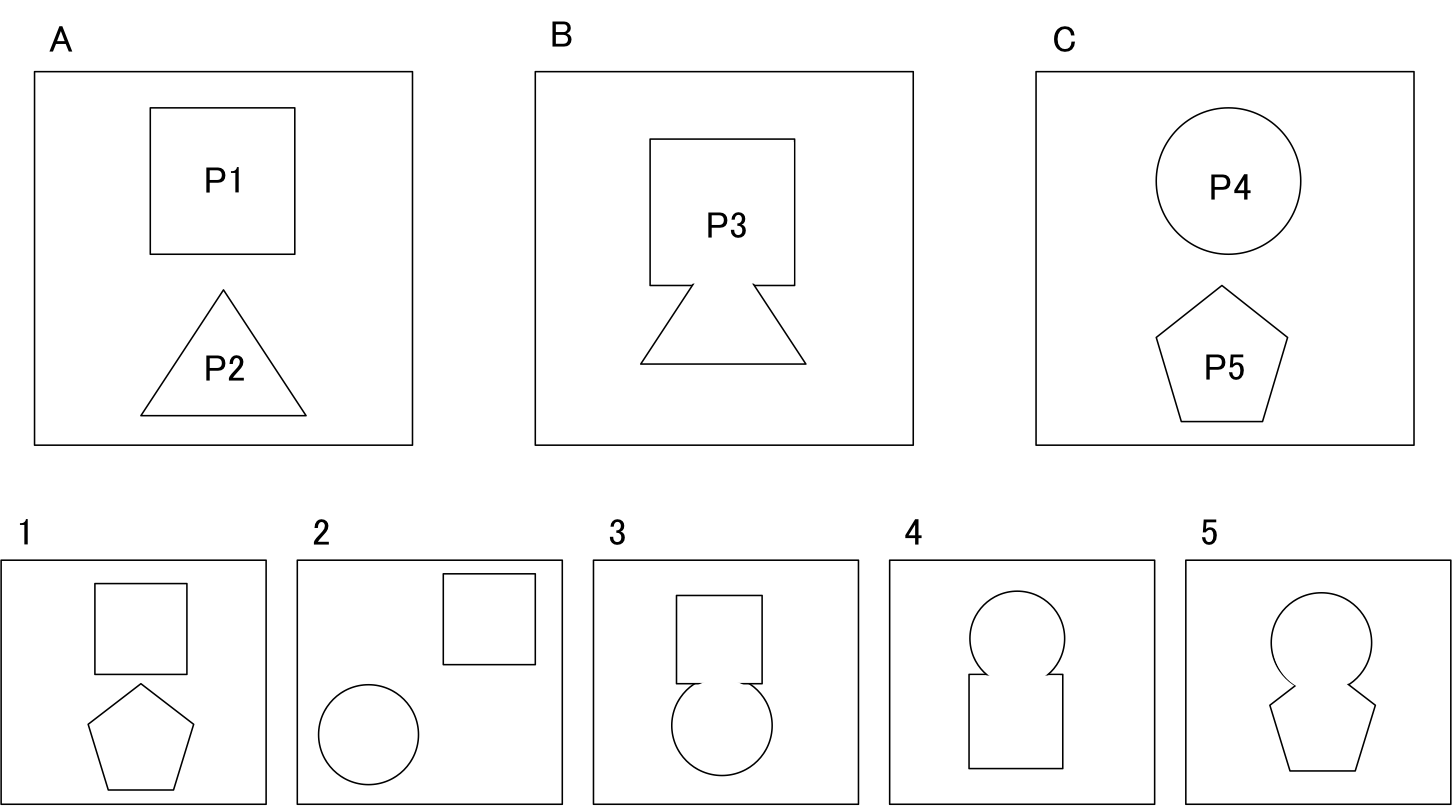
\includegraphics[width=13cm]{image/cant_solve.png}
	\caption{ANALOGYでは解けないであろう幾何図形類推問題(その1)}
	\label{fig:cant_solve}
	\end{center}
\end{figure}

EvansのANALOGYでは,まずA,B,Cの規則をそれぞれ記述するが,その際に,図に含まれるオブジェクトごとにその形やオブジェクトとの関係を記述する.そして,A,B間,A,C間でオブジェクトの対応(類似関係)を記述する.この記述は,一対一のオブジェクトで対応させる.このとき,多対一や多対多であると,変換規則を一意に定められないのは明らかである.

しかし,図\ref{fig:cant_solve}のBのようにAの図形を2つ接合してしまうと,AとBのオブジェクトに一対一の対応をつけることができない.したがって,ANALOGYはその変換規則を正しく記述できないため,問題が解けないと推察される.

これを実際に確かめてみる.この際のA,B,Cの記述は,例えばリスト\ref{code:cant_solve_description}になると考えられる.
\lstset{style=customplain}
\lstinputlisting[caption={A,B,Cの記述},label=code:cant_solve_description]{source/cant_solve_description.txt}



類似関係の記述は,A,B間では同じ図形はなく,A,C間にもないため記述はない.続いて,変換規則を記述するが,これはリスト\ref{code:cant_solve_description}からわかるように,AとBに一対一の対応が無いため機械的に記述できない.よって,変換規則が導出できないため,この問題は解決できない.

ここで,類似関係を意図的に記述することを考えると,一対一の対応を取るために「P1がP3に変形された」か「P2がP3に変形された」のどちらかが記述できる.すると,変換規則は,それぞれ「P1に三角形を重ね,P2を削除する」か,「P2に四角形を重ね,P1を削除する」という記述が機械的に得られる.しかし,これをCに適用しても,それぞれ「P4に三角形を重ね,P5を削除する」か「P5に四角形を重ね,P4を削除する」のいずれかとなって,正しい答えは導かれない.これは,図形の合成を新しい記述として取り入れても,一対一の関係を守る以上は解くことができない.

この他に,図\ref{fig:cant_solve_2}のような問題も解くことができないと考えられる.この問題はAで示された点の数がBの図形の頂点数に対応する.したがって,Cの図形は4の六角形へと変換される.この問題では,図形の類推の他に数え上げの機能を必要とするのは明らかである.しかし,ANALOGYはそのような機能を備えていないため,問題を解くことが出来ないと言える.
\begin{figure}[H]
	\begin{center}
	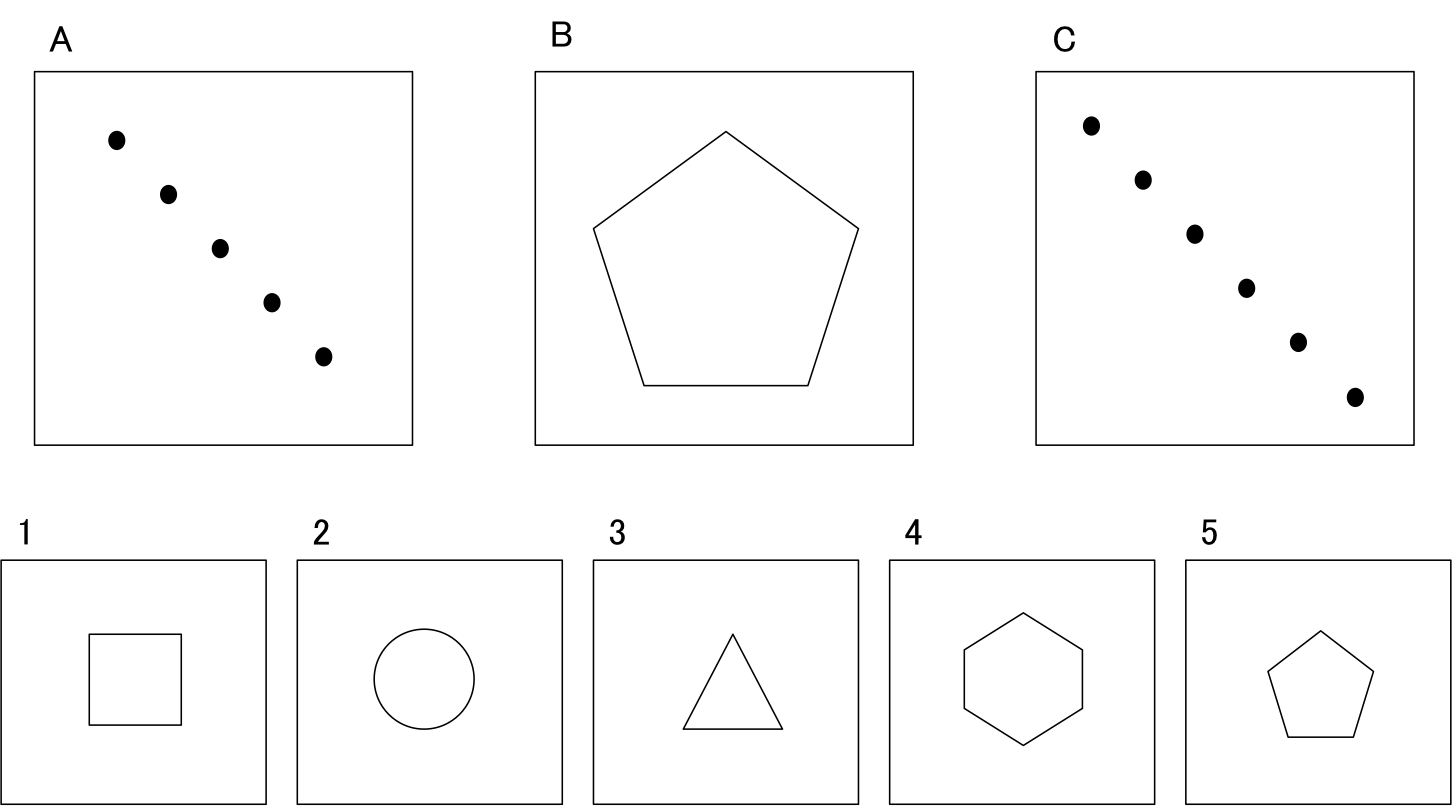
\includegraphics[width=13cm]{image/cant_solve_2.png}
	\caption{ANALOGYでは解けないであろう幾何図形類推問題(その2)}
	\label{fig:cant_solve_2}
	\end{center}
\end{figure}

その他,そもそもAとBが全く異なる図についてはANALOGYは答えを求められない.結局のところ,ANALOGYにどのような機能をもたせるべきかというフレーム問題を考えなければならないことがわかる.






\subsection{幾何図形類推問題の命題}
%EvansのプログラムANALOGYとIQテストに用いられるような幾何図形類推問題に関する以下の命題について、上で示した例などを利用して論ぜよ。
今までの内容を踏まえ,以下の2つの命題について考える.



\subsubsection{幾何学的図形類推問題を解く知的行為の基本的な要素は,純粋に機械的なものであることを示した}
\label{sec:thesis1}
幾何学的図形類推問題を解く知的行為は,純粋に機械的にできるものではないと考える.

ANALOGYは,図の記述と類似関係(変換規則)を手動で与えることで解を求めるプログラムであった\cite{ref:automation}.これが全て機械的な操作で記述できると仮定してみる.

前述の例で,Cの記述を変えると変換結果が変わり,正解が異なることが示された.これは,様々な手法により最も適する図の記述を類推することで解決できると考えられるが,それは「どのような制約条件を与えて記述を最適化するか」という問題に行き当たる.しかし,機械では制約条件を導くことができない.なぜなら,制約条件を与えるための条件が必要となり,さらにその条件を与えるための条件が必要になるというように,条件を定める責任をどこかに求めなければいけないからである.すると,ここでヒューリスティックな手法で条件を与える必要が出てくる.よって,機械的な手法だけでは幾何学的図形類推問題を解くことは出来ない.

また,\ref{sec:cant_solve}節で,ANALOGYという幾何学的図形類推問題を解くプログラムでは解けない問題があることを示した.この節の最初の例では,2つの図形と,それらを合成した図形との対応をA,B間で記述できないことが問題であると述べた.これは,もとになる記号的記述体系さえ適切に決めることができれば解消できる問題であった.

しかし,次の例である「図形の数を数え上げて,その数と同じ頂点数を持つ図形を選ぶ」という問題では,単に図形が変形したことが記述できるだけでなく,数え上げの機能が必要であること示した.

人間であれば,問題に直面した際に,その問題に適した手順と記述を使い分けることができる.前述の例であれば,図形の数と頂点数が対応していそうだと判断した場合は,数を数えてそれを記述することで問題を解き,図形の変形や消失などのみで類推が行える場合は,その問題に適するように変形の規則を記述できる.重要なことは,問題に直面した際にどの記述を選び,適用するのかということである.結局,この部分で,ヒューリスティックな手法を用いることになり,機械的な操作のみでは正解を導くことが出来ない.

よって,「幾何学的図形類推問題を解く知的行為の基本的な要素は,純粋に機械的なものであることを示した」とは言えないと考える.





\subsubsection{幾何学的図形類推問題を解くのに必要な知的な能力は,もとになる記号的記述体系をどのように選ぶかというところにのみ存在する}
記号的記述体系を選ぶ方法を決めるだけでは幾何学図形類推問題を解くのに十分であるとは言えないと考える.

\ref{sec:thesis1}節で,ヒューリスティックな方法で,もとになる記述を選ぶ必要があると述べた.しかし,記述を選ぶことだけで事足りるのだろうか.

\ref{sec:cant_solve}節の2つ目の問題をもう一度扱うと,この問題では,図形の類推において,数え上げの機能が必要である.しかし,単に数え上げの機能が必要であるだけでなく,数字とある図形を対応付ける知識も持っていなければならない.例えば,その数は図形の辺の数なのか,頂点数なのか,またその図形は全ての辺の長さが同じでなければならないのか,異なっても良いのかなど様々な条件を含めて考える必要がある.

この他にも,様々な類推方法が考えられ,それぞれにあった記述を作る必要がある.つまり,記述を選ぶ能力だけでなく,どのような記述方法を持っているかが重要となる.記述を選ぶためには,選ばれる記述がないといけないのである.したがって,様々な問題を想定して,記述方法を用意して置かなければならない.

では,どれだけ多くの記述方法を用意しておけばよいのだろうか.これは,どのような問題を幾何学的図形類推問題として想定するかというフレーム問題に帰着する.想定される問題の種類が多すぎて,列挙しきれないため,どのような記述を用意すればよいかわからない.またそれは,どの記述を選べばよいかわからないという問題にもつながる.これによって,あらゆる問題に対応した知識を持つことが難しくなるのである.

よって,幾何学的図形類推問題を解くのに必要な知的な能力として,「もとになる記号的記述体系をどのように選ぶか」に加え,「もとになる記号的記述体系をどのように用意するか」が想定される.




\begin{thebibliography}{n}
\bibitem{ref:book}
伊庭 斉志 :『人工知能と人工生命の基礎』,オーム社 (2013.5.24)

\bibitem{ref:automation}
藤井 智之 :『幾何図形上のアナロジー推論の自動化に関する研究』(last accessed at 2013.11.19),\url{http://ir.c.chuo-u.ac.jp/repository/search/item/md/typ/p/2559/}

\end{thebibliography}

\end{document}












